\documentclass[11pt,a4paper]{article}

\usepackage[margin=2.5cm]{geometry}
\usepackage{graphicx}
\usepackage{booktabs}
\usepackage{amsmath,amssymb}
\usepackage{xcolor}
\usepackage{enumitem}
\usepackage{caption}
\usepackage{hyperref}
\usepackage{fancyhdr}
\usepackage{titlesec}

% --- Colours ---
\definecolor{accent}{HTML}{2d3436}

% --- Header/footer ---
\pagestyle{fancy}
\fancyhf{}
\rhead{\small Girish Narayanan}
\lhead{\small LCAS --- Weekly Report}
\rfoot{\small\thepage}
\renewcommand{\headrulewidth}{0.4pt}

% --- Experiment environment ---
\newcounter{expnum}
\newenvironment{experiment}[1]{%
  \refstepcounter{expnum}%
  \subsection*{Experiment \theexpnum: #1}%
  \vspace{-0.5em}%
}{\vspace{1em}}

\newcommand{\setup}[4]{%
  \noindent
  \begin{tabular}{@{}p{2.8cm}p{11cm}@{}}
    \toprule
    \textbf{Variables}    & #1 \\
    \textbf{Constraints}  & #2 \\
    \textbf{Residual}     & #3 \\
    \textbf{Solver}       & #4 \\
    \bottomrule
  \end{tabular}
  \vspace{0.8em}
}

% --- Section styling ---
\titleformat{\section}{\large\bfseries\color{accent}}{}{0em}{}[\vspace{-0.3em}\rule{\textwidth}{0.4pt}]

\begin{document}

% ============================================================
% TITLE
% ============================================================
\begin{center}
  {\LARGE\bfseries Winding Ambiguity in $\boldsymbol{\omega}$ Bridging}\\[0.5em]
  {\large Weekly Report --- 10 March 2026}\\[0.3em]
  Girish Narayanan
\end{center}
\vspace{1em}

% ============================================================
\section{Context}

Test case: IS-901.\;
$\boldsymbol{\omega}_\text{true} = (0.5,\,-0.3,\,2.0)\,^\circ/\text{s}$,\;
$|\boldsymbol{\omega}_\text{true}| = 2.083\,^\circ/\text{s}$.

Experiments~1--4 use a 120\,s window (100 observations, $\Delta t_\text{samp} \approx 1.21\,$s, $\sigma = 0.05$\,mag).
Experiments~5--6 use a 3600\,s window (500 observations) with brightness peaks at indices 183, 260, 360.

% ============================================================
\section{Experiments}

% --- Exp 1 ---
\begin{experiment}{Forward Propagation --- Analytic $\boldsymbol{\omega}$, Exact Attitude, Hi-fi}

\setup
  {None (no free parameters)}
  {IS-901; $q_{k-1}, q_k$ exact from true trajectory; initial orientation: $160^\circ$ about arbitrary axis; hi-fi shadowing}
  {MSE between reconstructed and observed LC (computed, not optimised)}
  {None --- $\boldsymbol{\omega} = \mathrm{rotvec}(q_{k-1}^{-1}\, q_k) / \Delta t_\text{samp}$ (analytic, two consecutive observations); Euler forward propagation from $q_k$}

\textbf{Result:} Reconstructed LC overlays truth. At $\Delta t_\text{samp} \approx 1.21\,$s the axis-angle estimate recovers $\boldsymbol{\omega}$ to $< 10^{-6}\,^\circ/\text{s}$ error because the rotation between consecutive observations ($\sim$2.5$^\circ$) has no winding ambiguity.

\begin{figure}[h]
  \centering
  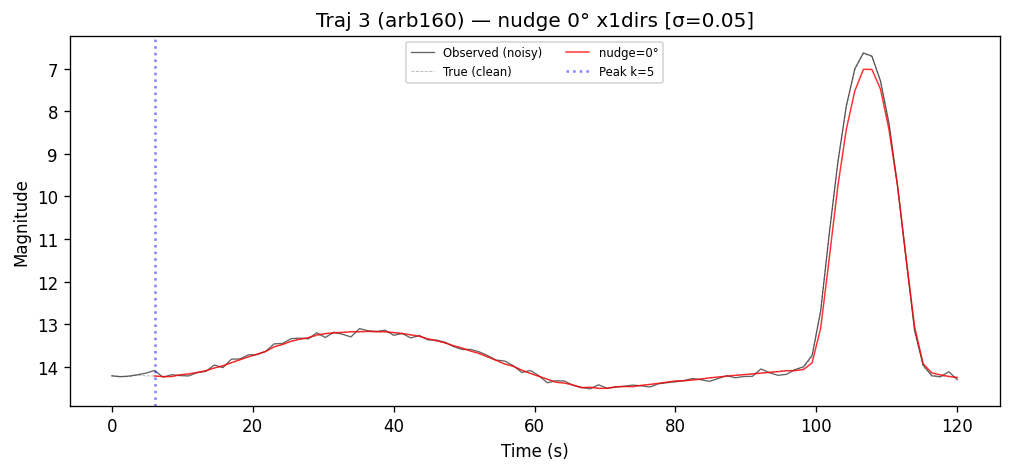
\includegraphics[width=0.85\textwidth]{../../data/results/inversion_diagnostics/micro01b_qnudge_2.08dps_traj3_nudge0.png}
  \caption{Hi-fi forward propagation from exact $q_k$ with analytic $\boldsymbol{\omega}$ (trajectory~3, arb160). Red overlays truth.}
\end{figure}

\end{experiment}

% --- Exp 2 ---
\begin{experiment}{Forward Propagation --- Analytic $\boldsymbol{\omega}$, 3$^\circ$ Attitude Nudge, Hi-fi}

\setup
  {Nudge direction (5 random unit vectors, deterministic seed 123; not optimised)}
  {Same analytic $\boldsymbol{\omega}$ as Exp~1 (from exact $q$); $q_k$ nudged $3^\circ$ before propagation; hi-fi shadowing}
  {MSE per direction (computed, not optimised)}
  {None --- same analytic $\boldsymbol{\omega}$; Euler forward propagation from nudged $q_k$}

\textbf{Result:} Sensitivity is anisotropic. Near the glint ($t \approx 107\,$s), some nudge directions barely change the LC; others shift the peak by $>$2\,mag.

\begin{figure}[h]
  \centering
  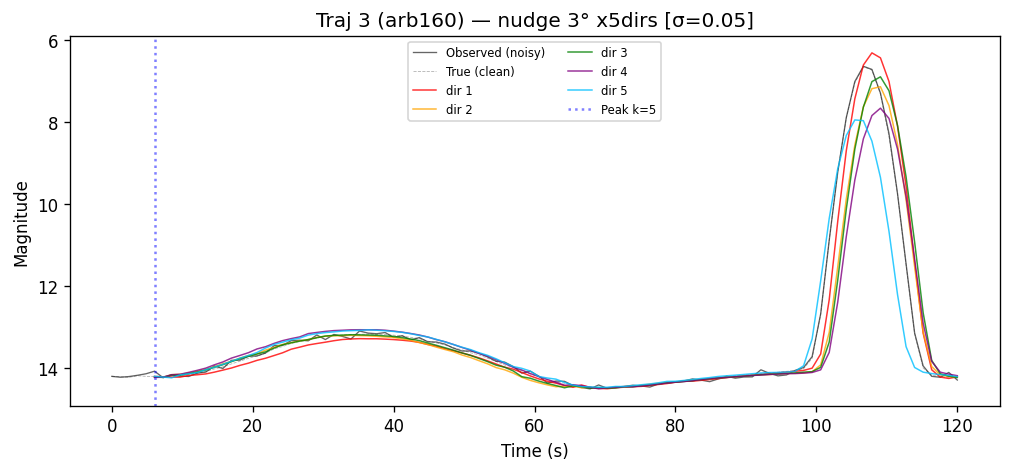
\includegraphics[width=0.85\textwidth]{../../data/results/inversion_diagnostics/micro01b_qnudge_2.08dps_traj3_nudge3.png}
  \caption{Hi-fi forward propagation from 3$^\circ$-nudged $q_k$ in 5 directions (trajectory~3, arb160).}
\end{figure}

\end{experiment}

% --- Exp 3 ---
\begin{experiment}{Forward Propagation --- Analytic $\boldsymbol{\omega}$, Exact Attitude, Lo-fi Reconstruction}

\setup
  {None}
  {Same analytic $\boldsymbol{\omega}$ and exact $q_k$ as Exp~1; reconstruction uses lo-fi (no self-shadowing); observed LC is hi-fi; orientation: arb160}
  {MSE(lo-fi reconstruction, hi-fi observed)}
  {None --- forward evaluation only}

\textbf{Result:} Lo-fi predicts a bright glint at $t \approx 60\,$s that does not exist in the hi-fi observations. At this orientation a facet is in self-shadow; hi-fi suppresses it, lo-fi does not.

\begin{figure}[h]
  \centering
  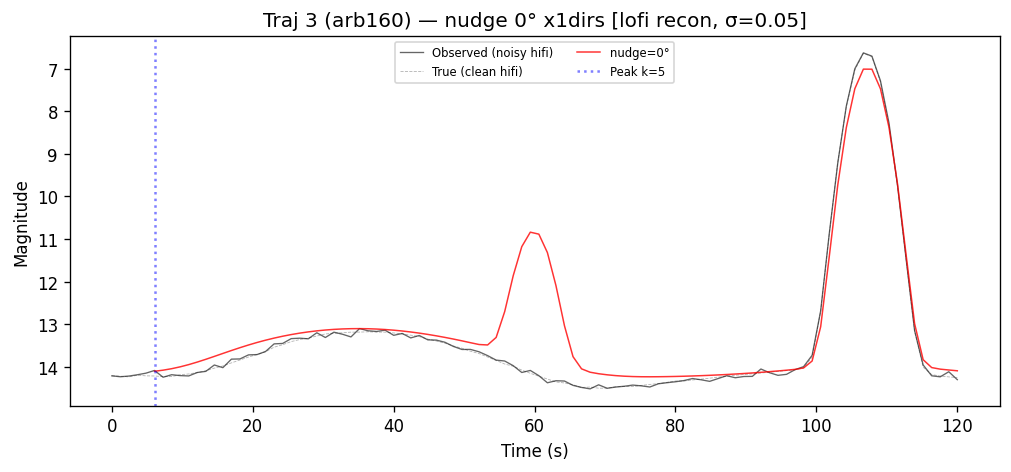
\includegraphics[width=0.85\textwidth]{../../data/results/inversion_diagnostics/micro01c_lofi_qnudge_2.08dps_traj3_nudge0.png}
  \caption{Lo-fi reconstruction (no shadows) vs hi-fi observed (trajectory~3, arb160). Phantom peak at $t \approx 60\,$s.}
\end{figure}

\end{experiment}

% --- Exp 4 ---
\begin{experiment}{Forward Propagation --- Analytic $\boldsymbol{\omega}$, 3$^\circ$ Nudge, Lo-fi (Different Orientation)}

\setup
  {Nudge direction (5 random unit vectors)}
  {Same analytic $\boldsymbol{\omega}$; $q_k$ nudged $3^\circ$; lo-fi reconstruction; orientation: $30^\circ$ about $\hat{x}$}
  {MSE(lo-fi reconstruction, hi-fi observed) per direction}
  {None --- forward evaluation only}

\textbf{Result:} No phantom peak. Lo-fi and hi-fi agree at this orientation. The lo-fi failure in Exp~3 occurs only at orientations with active self-shadowing and cannot be predicted a priori.

\begin{figure}[h]
  \centering
  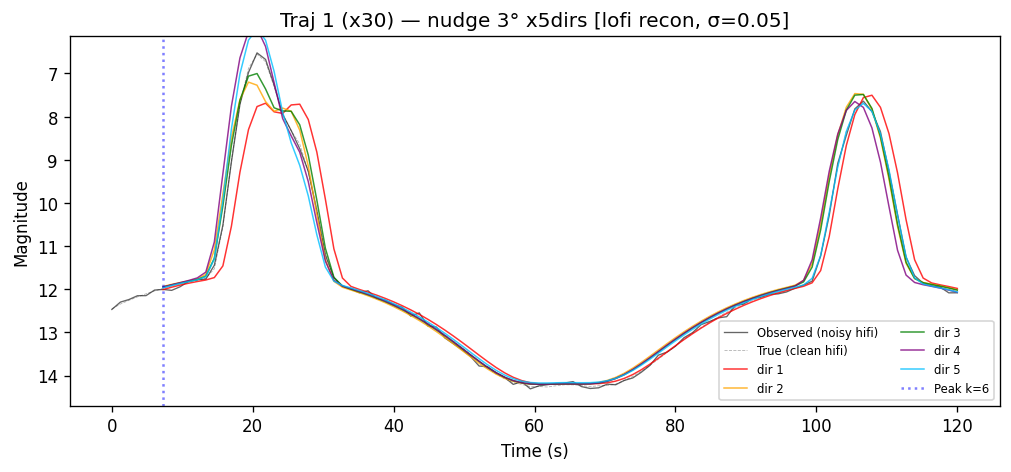
\includegraphics[width=0.85\textwidth]{../../data/results/inversion_diagnostics/micro01c_lofi_qnudge_2.08dps_traj1_nudge3.png}
  \caption{Lo-fi reconstruction at benign orientation (trajectory~1, x30). No phantom peak.}
\end{figure}

\end{experiment}

\clearpage

% --- Exp 5 ---
\begin{experiment}{Staircase $\boldsymbol{\omega}$ Enumeration via Barrier-Constrained Optimisation}

\setup
  {$\boldsymbol{\omega} \in \mathbb{R}^3$ (optimised per step)}
  {$q_A, q_B$ exact (oracle) at peaks 183, 260; $\Delta t = 555.5\,$s; soft lower barrier on $|\boldsymbol{\omega}|^2$ incremented after each step to force progression through winding bands}
  {Optimisation objective: $1 - (q_\text{prop} \cdot q_B)^2 + \lambda_\text{barrier}$;\; post-hoc trough score: $|b_\text{pred} - b_\text{ref}|$ (lo-fi, single epoch between peaks)}
  {L-BFGS-B, 8 sequential steps; step~0 init: axis-angle $\mathrm{rotvec}(q_A^{-1}\,q_B)/\Delta t$; subsequent steps init: previous $\boldsymbol{\omega}$ + one extra revolution along rotation axis}

\textbf{Result:}

\begin{center}
\begin{tabular}{cccl}
  \toprule
  Step & $|\boldsymbol{\omega}|\;(^\circ/\text{s})$ & Arrival err & Trough err \\
  \midrule
  0 & 0.316 & 0.0 & 1.719 \\
  1 & 0.959 & 0.0 & 0.099 \\
  2 & 1.601 & 0.0 & 0.021 $\leftarrow$ best trough \\
  \textbf{3} & \textbf{2.230} & \textbf{0.0} & 0.792 $\leftarrow$ \textbf{true} ($|\boldsymbol{\omega}_\text{true}| = 2.083$) \\
  4 & 2.883 & 0.036 & 0.044 \\
  5 & 3.509 & 0.0 & 0.134 \\
  6 & 4.180 & 0.0 & 1.749 \\
  7 & 4.824 & 0.0 & 1.491 \\
  \bottomrule
\end{tabular}
\end{center}

Staircase successfully enumerates 8 distinct winding solutions. Trough scoring (lo-fi, single epoch) selects step~2 (wrong)---at the trough epoch, steps~2 and~3 have not diverged enough to produce a detectable brightness difference.

\end{experiment}

% --- Exp 6 ---
\begin{experiment}{Angular Momentum Conservation Filter --- Two-Leg Staircase}

\setup
  {$\boldsymbol{\omega} \in \mathbb{R}^3$ per leg per step (optimised independently)}
  {$q_A, q_\text{mid}, q_B$ exact (oracle) at peaks 183, 260, 360; leg~0 $\Delta t = 555.5\,$s; leg~1 $\Delta t = 721.4\,$s; lower + upper $|\boldsymbol{\omega}|$ barriers per step ($\pm 0.8\,\delta$ band)}
  {Per step: $1 - (q_\text{prop} \cdot q_\text{end})^2$ + barrier penalties;\; L-filter: $\|\mathbf{L}_{\text{leg\,0}}[k] - \mathbf{L}_{\text{leg\,1}}[j]\|$ where $\mathbf{L} = R(q_\text{mid})\,I\,\boldsymbol{\omega}$}
  {L-BFGS-B per step (with barriers); exhaustive $8 \times 8 = 64$ L-comparison at shared peak~260}

\textbf{Result:} Filter selected $(k{=}0,\, j{=}0)$. True pair: $(k{=}3,\, j{=}1)$. \textbf{Incorrect}---leg~1 staircase is broken.

\begin{center}
\begin{tabular}{ccc}
  \toprule
  Step & Leg\,0 $|\boldsymbol{\omega}|\;(^\circ/\text{s})$ & Leg\,1 $|\boldsymbol{\omega}|\;(^\circ/\text{s})$ \\
  \midrule
  0 & 0.316 & 0.249 \\
  1 & 0.959 & 3.279 $\leftarrow$ gap \\
  2 & 1.601 & 3.509 \\
  3 & 2.230 & 3.995 \\
  \bottomrule
\end{tabular}
\end{center}

Leg~0 steps uniformly ($\sim$+0.65$\,^\circ$/s per step). Leg~1 jumps from 0.249 to 3.279, skipping winding bands 1--3. Cause: axis-angle init for leg~1 lands near a $\pi$-rotation; quaternion double-cover causes discontinuous jump. Fix: initialise from $\boldsymbol{\omega}_0 = \mathbf{0}$, tighten upper barrier.

\end{experiment}

% ============================================================
\section{Decisions}

\begin{itemize}[nosep]
  \item MIP/integer programming ruled out (consulted Jack---insufficient discrete structure).
  \item Lo-fi cannot be used for scoring near glints (Exp~3--4). Hi-fi required.
  \item Single-trough scoring insufficient (Exp~5). Need multi-epoch or physics-based filter.
  \item Angular momentum conservation is the most promising $\omega$ filter (Exp~6), pending staircase fix.
\end{itemize}

% ============================================================
\section{Next Steps}

\begin{enumerate}[nosep]
  \item Fix staircase seed ($\boldsymbol{\omega}_0 = \mathbf{0}$ + tight upper barrier) for leg~1.
  \item Rerun L-conservation filter with fixed staircase.
  \item Test with approximate endpoints ($2$--$5^\circ$ attitude error).
  \item Stack multiple troughs as secondary discriminator.
\end{enumerate}

\end{document}
